% =============================================================================
% paper_v1.tex - ICU-Sepsis OOD-action study (NeurIPS 2026 format, DOUBLE-BLIND)
%
% v1 EXECUTOR FILL-IN, 2026-05-23. Derived from main.tex; Method + Experiments
% reused, and Abstract / Introduction / Related Work / Discussion / Conclusion
% prose written out. Blueprints: core_docs/paper_spec.md (read the top "v1
% decisions" block, then 0.0/0.3/per-section), core_docs/spec.md (format).
%
% CROSS-ALGORITHM RESULTS: saved policies from the released experimental pipeline
% are re-evaluated EXACTLY against the true dynamics via the saved-policy evaluation script, so every trained value is <= V*.
%
% TO COMPILE (Overleaf): drop neurips_2026.sty into the project. Anonymous
% submission mode (do NOT pass [final]) auto-prints "Anonymous Author(s)" and
% enables line numbers. The six PNGs live in submission/figures/ (graphicspath
% below also looks in ./figures/).
% ANONYMITY: no names / affiliations / identifying URLs in the PDF. The code link
% in the Reproducibility statement is an anonymized anonymous.4open.science mirror.
% =============================================================================
\documentclass{article}
\usepackage{neurips_2026}    
\usepackage{float}          
\usepackage[utf8]{inputenc}
\usepackage[T1]{fontenc}
\usepackage{hyperref}
\usepackage{url}
\usepackage{booktabs}
\usepackage{amsfonts}
\usepackage{amsmath}
\usepackage{amssymb}
\usepackage{graphicx}
\usepackage{microtype}
\usepackage{xcolor}
\usepackage{enumitem} % for enumerate [leftmargin=...] options
\usepackage{nicefrac}    
% Self-contained: all figures live in ./figures/ (this folder).
\graphicspath{{figures/}}

\newcommand{\Adm}{\mathcal{A}_{\mathrm{adm}}}
\newcommand{\dist}{\mathrm{dist}\text{-}V^\star}
\newcommand{\todo}[1]{\textcolor{red}{[TODO: #1]}}

\title{When Mean Imputation Hides Unsupported Actions:\\
Diagnosing an Out-of-Distribution Action\\
Failure Mode in the ICU-Sepsis Benchmark}

\author{%
  Anonymous Author(s)\\
  Affiliation\\
  \texttt{email}\\
}

\begin{document}
\maketitle

\begin{abstract}
ICU-Sepsis exposes a rare opportunity to audit offline-RL action-support failures
exactly: although it is distilled from real ICU trajectories, it ships tabular
dynamics and therefore allows exact evaluation against the optimal value
$V^\star$. We use this property to test the benchmark's default \texttt{mean}
imputation rule, which replaces every data-unsupported action with the average
transition of the supported actions in that state. Although this rule is described
as equivalent to choosing a random admissible action, we find that it creates a
hidden failure mode for model-free RL: vanilla Q-learning selects unsupported
actions in $\sim$87\% of states and reaches $J{=}0.785$, no better than the Random
(0.780) and clinician (0.782) baselines and far below the optimal value
($J^\star{=}0.875$).

A component ablation localizes the mechanism. Masking unsupported actions only at
deployment removes invalid deployed actions but leaves the learned $Q$-table
corrupted, with $Q$-value leakage unchanged at $+0.46$. In contrast, restricting
the behavior policy during training matches the full support mask and reduces the
value gap from $0.090$ to $0.069$. Additional support-aware remedies---soft
penalties, CQL-style conservatism, cross-algorithm checks, and a finite-data
offline empirical-MDP study---support the same conclusion: the issue is not the
final deployed action alone, but sampling and bootstrapping unsupported actions
during learning. Our results are benchmark-internal, not clinical
recommendations. The transferable takeaway is an exact-$V^\star$ auditing
protocol: ICU-Sepsis results should report how inadmissible actions are handled,
together with deployed-unsupported rate, value gap, and leakage diagnostics.
\end{abstract}

% =============================================================================
\section{Introduction}
\label{sec:intro}
Offline medical reinforcement learning (RL) is shaped by uneven action support:
some treatments are well represented in the logged data, while others are rarely
or never observed in a given clinical state. How an RL benchmark handles these
low-support actions is therefore not a harmless implementation detail. It can
change what a learner samples, bootstraps from, and ultimately deploys.

ICU-Sepsis \citep{choudhary2024icusepsis} is a useful testbed for this question
because it is both clinically motivated and exactly evaluable. The benchmark is a
tabular sepsis-treatment MDP distilled from MIMIC-III trajectories, and it ships
its full transition dynamics. Unlike most medical RL settings, where policy
quality must be estimated through noisy off-policy evaluation
\citep{gottesman2019guidelines,gottesman2018evaluating}, ICU-Sepsis lets us
compute the optimal value $V^\star$ and the exact value of any learned policy.
We use this exact value not as a leaderboard target, but as a measurement
instrument for diagnosing action-support failures.

We focus on the benchmark's default \texttt{mean} imputation strategy. In each
state, ICU-Sepsis identifies an admissible set $\Adm(s)$ of sufficiently supported
actions. For every inadmissible action, the default strategy replaces its
transition with the average transition over admissible actions. The benchmark
motivates this as ``equivalent to choosing a random admissible action.'' We show
that this equivalence hides a measurable cost: under the default dynamics,
vanilla Q-learning selects unsupported actions in $\sim$87\% of states while
achieving only random/clinician-level value. Numerically, its exact
$d_0$-weighted value (the survival probability) is $J{=}0.785$, close to the
Random (0.780) and clinician (0.782) baselines and far below the optimal value
$J^\star{=}0.875$.

The central finding is mechanistic. The obvious fix---masking unsupported actions
only when extracting the final policy---is insufficient. It drives the deployed
unsupported-action rate to zero, but does not repair the learned $Q$-values. We
quantify this residual corruption with $Q$-value leakage: the extent to which the
best unsupported action is valued above the best supported action. Under
deployment-only masking, this leakage remains at $+0.46$---essentially unchanged
from vanilla Q-learning---so the final policy appears admissible while the
learned value estimates remain contaminated. In our component ablation, the
decisive intervention is instead \emph{behavior-level} support control:
unsupported actions must be kept out of the training behavior that is sampled and
bootstrapped. This behavior-only mask matches the full support mask and improves
the exact value gap to $V^\star$ from $0.090$ to $0.069$.

\paragraph{Contributions.}
\begin{enumerate}[leftmargin=2em,itemsep=2pt,topsep=2pt]
  \item \textbf{A hidden benchmark failure.} We show that ICU-Sepsis's default
  mean-imputation rule makes unsupported actions appear average, causing vanilla
  model-free agents to select them in $\sim$87\% of states while achieving only
  random/clinician-level value (\S\ref{sec:failure}).
  \item \textbf{A mechanism-level diagnosis.} A component ablation and exact
  $Q$-value-leakage diagnostic show that the failure comes from behavior-level
  sampling, not merely from the final deployed policy (\S\ref{sec:mechanism}).
  \item \textbf{A support-aware auditing protocol.} We corroborate this conclusion
  across a spectrum of support-aware interventions, including soft penalties,
  conservative regularization, admissibility masking, cross-algorithm checks, and
  finite-data offline experiments. These results suggest that ICU-Sepsis reports
  should state how inadmissible actions are handled, together with deployed
  unsupported-action rate, value gap to $V^\star$, and leakage/overestimation
  diagnostics (\S\ref{sec:remedy}--\S\ref{sec:offline}).
\end{enumerate}

% =============================================================================
\section{Related Work}
\label{sec:related}
\paragraph{Medical RL benchmarks.}
Sepsis treatment has been a recurring testbed for RL in healthcare
\citep{komorowski2018aiclinician,raghu2017continuous}, but learning from logged
clinical data is hampered by unknown dynamics and unreliable evaluation.
ICU-Sepsis \citep{choudhary2024icusepsis} and related curated benchmarks
\citep{mimic_sepsis_arxiv2510_24500} distill such data into reproducible MDPs.
Our work differs by treating such a benchmark as a \emph{measurement instrument}
for a specific pathology---using its exact $V^\star$ to audit how data-unsupported
actions are handled---rather than as a leaderboard to top.

\paragraph{Offline RL and OOD actions.}
The danger of bootstrapping from out-of-distribution actions, and the resulting
value overestimation, is the motivating problem for batch-constrained,
behavior-regularized, and conservative offline methods
\citep{fujimoto2019bcq,kumar2019bear,kumar2020cql}, with pessimism shown to be
provably and practically effective \citep{rashidinejad2021pessimism,jin2021pessimism}.
Our work differs by measuring this recognized pathology \emph{exactly} against
ground-truth $V^\star$ in an environment distilled from real data, isolating where
in the learning update the failure originates.

\paragraph{Invalid / forbidden action masking.}
Masking unavailable actions is standard in deep RL, both as an analysis target in
policy-gradient methods \citep{huang2021masking} and as a way to learn from
forbidden actions \citep{seurin2020forbidden}, and is available off-the-shelf as
maskable policies \citep{raffin2021sb3}. We
do not introduce masking; instead, a component ablation shows precisely \emph{where}
it must act---at the behavior level---and that masking only the target or only the
deployed policy is insufficient.

\paragraph{Tabular model-based RL.}
For small tabular MDPs, optimism- and posterior-sampling-based model-based methods
are known to be near-optimal \citep{auer2008ucrl,osband2013psrl}. We
\emph{acknowledge} that a $716$-state model-based agent reaching $V^\star$ is
expected, not a feat; we therefore frame our model-based remedy as the endpoint of
a spectrum that demonstrates the gap is an artifact of mean-imputation, and our
contribution is the diagnosis and mechanism, not a regret or optimality result.

\paragraph{Reward shaping and behavior-constrained learning.}
Potential-based reward shaping leaves the optimal policy invariant
\citep{ng1999reward}, which justifies our supplementary severity-based shaping;
constraining a learner toward a behavior policy is likewise a standard offline-RL
device \citep{wu2019behavior,nair2020awac}.
Our work differs by using these only as supplementary points on the remedy
spectrum, with admissibility---not shaping---as the load-bearing structure.

\paragraph{Evaluation pitfalls in healthcare RL.}
Off-policy evaluation in observational health settings is noisy and easily
misleading \citep{gottesman2019guidelines,gottesman2018evaluating}. Our work
differs by sidestepping OPE entirely: exact $V^\star$ makes selection rates,
value gaps, and overestimation measurable in a way real cohorts do not allow.

% =============================================================================
\section{Background: ICU-Sepsis and Mean Imputation}
\label{sec:background}
ICU-Sepsis \citep{choudhary2024icusepsis} is a tabular MDP with $|\mathcal{S}|{=}716$
states (713 patient states plus death, survival, $s_\infty$) and $|\mathcal{A}|{=}25$
actions (5 fluid $\times$ 5 vasopressor levels). The reward is a survival indicator
(${+}1$ on transition into the survival state, $0$ otherwise) and $\gamma{=}1$, so
episodes are short and the undiscounted return equals the survival probability;
consequently $V^\star(s)$ is exactly the maximum achievable survival probability
from $s$. Because the full transition model is shipped with the benchmark, we
compute $V^\star$ and the exact value $V^\pi$ of any policy by value iteration,
avoiding off-policy estimation entirely. We write $d_0$ for the benchmark's
initial-state distribution and summarize a policy by its $d_0$-weighted value
$J(\pi)=\mathbb{E}_{s\sim d_0}[V^\pi(s)]$ (the survival probability), with
$J^\star=\mathbb{E}_{s\sim d_0}[V^\star(s)]$ the optimal value.

\paragraph{Admissibility and the \texttt{mean} strategy.}
Each state has an \emph{admissible} action set $\Adm(s)$: actions taken at least
$\tau{=}20$ times in the source cohort, so their transition estimates are reliable.
The remaining actions are \emph{inadmissible} (data-unsupported); admissible sets
are small (median 4, mean 3.2, of 25). For an inadmissible action $a\notin\Adm(s)$,
the benchmark's default \texttt{mean} strategy defines the transition as the
unweighted average over admissible actions:
\begin{equation}
\label{eq:mean}
P(s'\mid s,a) \;=\; \frac{1}{|\Adm(s)|}\sum_{a'\in\Adm(s)} \zeta(s,a',s'),
\qquad a\notin\Adm(s),
\end{equation}
where $\zeta$ is the empirical admissible-action transition. We verified
Eq.~\eqref{eq:mean} holds exactly in the shipped dynamics (every inadmissible row
equals the admissible mean to $7\times10^{-16}$). The benchmark motivates this as
``equivalent to choosing a random admissible action'' \citep{choudhary2024icusepsis};
\S\ref{sec:failure} shows this equivalence is precisely where the cost arises.

% =============================================================================
\section{Diagnostic Protocol and Support Controls}
\label{sec:method}
We frame inadmissible actions as out-of-distribution (OOD) / low-support actions
and use ICU-Sepsis's known dynamics to separate two questions: \emph{how large is
the hidden failure?} and \emph{where in the learning loop does it arise?} The
mechanism study uses tabular $Q:\mathcal{S}\times\mathcal{A}\to\mathbb{R}$
updates so that the effect of support control is not confounded by function
approximation. Broader agents and model-based results are used only as breadth
checks.

\paragraph{Exact diagnostics.}
We report three main diagnostics. First, the distance to optimal value is
$\dist(\pi)=\mathbb{E}_{s\sim d_0}[V^\star(s)-V^\pi(s)]$, where $V^\pi$ is
computed exactly by value iteration. Second, the deployed unsupported-action rate
is the fraction of non-terminal states in which the greedy policy selects
$a\notin\Adm(s)$. Third, $Q$-value leakage measures whether unsupported actions
are over-valued in the learned table:
\[
\frac{1}{|\mathcal{S}_{\mathrm{nt}}|}\sum_{s\in\mathcal{S}_{\mathrm{nt}}}
\left[\max_{a\notin\Adm(s)}Q(s,a)-\max_{a\in\Adm(s)}Q(s,a)\right].
\]
Positive leakage means unsupported actions are valued above the best supported
action on average. In the offline finite-data study we additionally report value
overestimation, defined as the empirical model's self-estimated value minus the
policy's exact value under the true benchmark dynamics.

\paragraph{Support-control interventions.}
The key ablation decomposes admissibility masking into three locations:
\textbf{behavior} masking restricts $\epsilon$-greedy exploration to $\Adm(s)$;
\textbf{target} masking restricts the Bellman backup maximum to $\Adm(s')$; and
\textbf{policy} masking restricts only the final greedy policy to $\Adm(s)$. Full
masking enables all three. This decomposition lets us test whether the pathology
comes from training-time sampling, bootstrapping, or final deployment.

We also include softer support-aware remedies as supporting comparisons. A
\emph{support penalty} subtracts $\lambda$ when an inadmissible action is sampled,
$r'(s,a,s')=r-\lambda\mathbb{1}[a\notin\Adm(s)]$. A \emph{CQL-style} tabular
regularizer nudges $Q(s,\cdot)$ toward the admissible support: at each visited
state it sets $Q(s,\cdot)\leftarrow Q(s,\cdot)-\alpha\kappa\big(\mathrm{softmax}(Q(s,\cdot))-u_{\Adm(s)}\big)$,
where $u_{\Adm(s)}$ is the distribution over all actions that is uniform on
$\Adm(s)$ and zero elsewhere. This is not a full CQL
implementation, but a conservative value-suppression test used only in tabular
$Q$-learning. Throughout, the
\emph{admissibility-aware} (AA) prefix denotes a learner whose admissible-action
mask is applied during learning (the AA-$\ast$ methods in Table~\ref{tab:merged}).
Finally, AA-MBRL serves as a model-based endpoint: it estimates an empirical transition
model and periodically solves value iteration restricted to $\Adm(s)$. We use
AA-MBRL only to show that the gap is largely an artifact of ignoring support and
model structure, not as a proposed algorithm or a fair model-free comparison.

% =============================================================================
\section{Experiments}
\label{sec:experiments}
\paragraph{Setup.}
Unless stated otherwise, mechanism experiments use 5 seeds,
$5{\times}10^4$ episodes, $\alpha{=}0.1$, $\gamma{=}1$, and
$\epsilon$ annealed from $1.0$ to $0.05$ over $10^4$ episodes.
The cross-algorithm and model-based comparisons in Table~\ref{tab:merged} use
$5{\times}10^5$ episodes. This larger budget does not explain the main failure:
vanilla Q-learning remains near the baseline at both budgets
($J{=}0.785$ at $5{\times}10^4$ and $J{=}0.787$ at
$5{\times}10^5$). We report means over 5 seeds; shaded bands in line plots show 95\% confidence
intervals across seeds, bar-chart error bars show $\pm$std, and the appendix
rollout curves use $\pm$1 SE (benchmark convention). Our conclusions rely not on
small survival-rate differences, but on support diagnostics with large effect
sizes.

\paragraph{Baselines reproduce the benchmark (Table~\ref{tab:baselines}).}
Exact $d_0$-weighted values match the published Random/Expert/Optimal numbers,
confirming that our exact-evaluation ruler is calibrated. Survival values also
occupy a narrow $0.78$--$0.875$ band, motivating our use of the exact value gap
$\dist$ alongside raw survival value.

\begin{table}[t]
\centering
\caption{Exact baseline reproduction ($d_0$-weighted policy value $=$ survival
rate). Values are computed by exact value iteration and are independent of the
training budget.}
\label{tab:baselines}
\begin{tabular}{lccc}
\toprule
 & Random & Clinician (Expert) & Optimal ($J^\star$) \\
\midrule
$J(\pi)$ & 0.780 & 0.782 & 0.875 \\
\bottomrule
\end{tabular}
\end{table}

\subsection{The hidden failure (Claim 1)}
\label{sec:failure}
Under the default \texttt{mean} strategy, vanilla Q-learning deploys
inadmissible actions in $\sim$87\% of states. Its exact value is
$J(\pi){=}0.785$ with $\dist{=}0.090$, essentially matching the Random
(0.780) and clinician (0.782) baselines. Applying admissibility control improves
the same learner to $J{=}0.806$ and $\dist{=}0.069$ at $5{\times}10^4$
episodes, showing that the gap is tied to
how unsupported actions are handled.

Crucially, this is not a mere labeling artifact. Under the \texttt{mean}
strategy, an inadmissible action behaves like a random admissible one
(Eq.~\eqref{eq:mean}). Selecting such an action therefore implements an
average-over-admissible transition. This can look competitive during
bootstrapping, but it prevents the learner from consistently recovering the best
admissible action, inducing a measurable value gap to $V^\star$. This is why
survival rate alone is not diagnostic: benchmark-style return metrics can look
plausible while $\dist$ and support-aware diagnostics reveal the hidden failure. The failure is also not specific to Q-learning or to a
small training budget: it persists across Sarsa/Q/DQN/PPO, and Q-learning remains
near the baseline level at $5{\times}10^5$ episodes ($J{=}0.787$ exact;
Table~\ref{tab:merged}).

\subsection{Mechanism: where the failure lives (Claim 2)}
\label{sec:mechanism}
A component ablation (Table~\ref{tab:ablation}; Fig.~\ref{fig:ablation})
localizes the failure to behavior-level support violations during learning. In
this ablation, behavior masking alone reproduces the full-mask result and is the
only component that reverses the positive $Q$-value leakage. The other masking locations help
only marginally: masking only the target leaves $\sim$77\% deployed unsupported
actions, while masking only the deployed policy drives deployment to zero but
does not repair the learned values, leaving leakage unchanged at $+0.46$.

The leakage diagnostic explains why. $Q$-value leakage flips from $+0.46$ under
vanilla Q-learning to $-0.80$ under behavior/full masking, showing that
unsupported actions become competitive only when they are sampled and updated
under mean-imputed dynamics. Fig.~\ref{fig:exactcurve} traces the same ordering
over training. We return to this sign interpretation in the remedy spectrum,
where overly negative leakage can indicate conservative over-suppression rather
than better value (\S\ref{sec:remedy}). The central mechanism result is therefore not that
unsupported actions should merely be suppressed, but that support must be
controlled at the behavior level during learning. The breadth experiments below
test whether this pattern persists beyond the ablation.

\begin{table}[t]
\centering
\caption{Component ablation over where admissibility masking is applied
(5 seeds, $5{\times}10^4$ episodes). Soft remedies such as CQL are covered
separately in the remedy spectrum (\S\ref{sec:remedy}).}
\label{tab:ablation}
\begin{tabular}{lcccl}
\toprule
Variant & $\dist\,\downarrow$ & Deploy unsupp. & Q-leakage & Reading \\
\midrule
vanilla            & 0.090 & 0.87 & $+0.46$ & unsupported over-valued \\
target-only        & 0.085 & 0.77 & $+0.07$ & backup alone insufficient \\
policy-only        & 0.083 & 0.00 & $+0.46$ & band-aid; $Q$ corrupted \\
\textbf{behavior-only} & \textbf{0.069} & 0.00 & $-0.80$ & reproduces full-mask result \\
full mask          & 0.069 & 0.00 & $-0.80$ & no additional gain \\
\bottomrule
\end{tabular}
\end{table}

\begin{figure}[tb]\centering
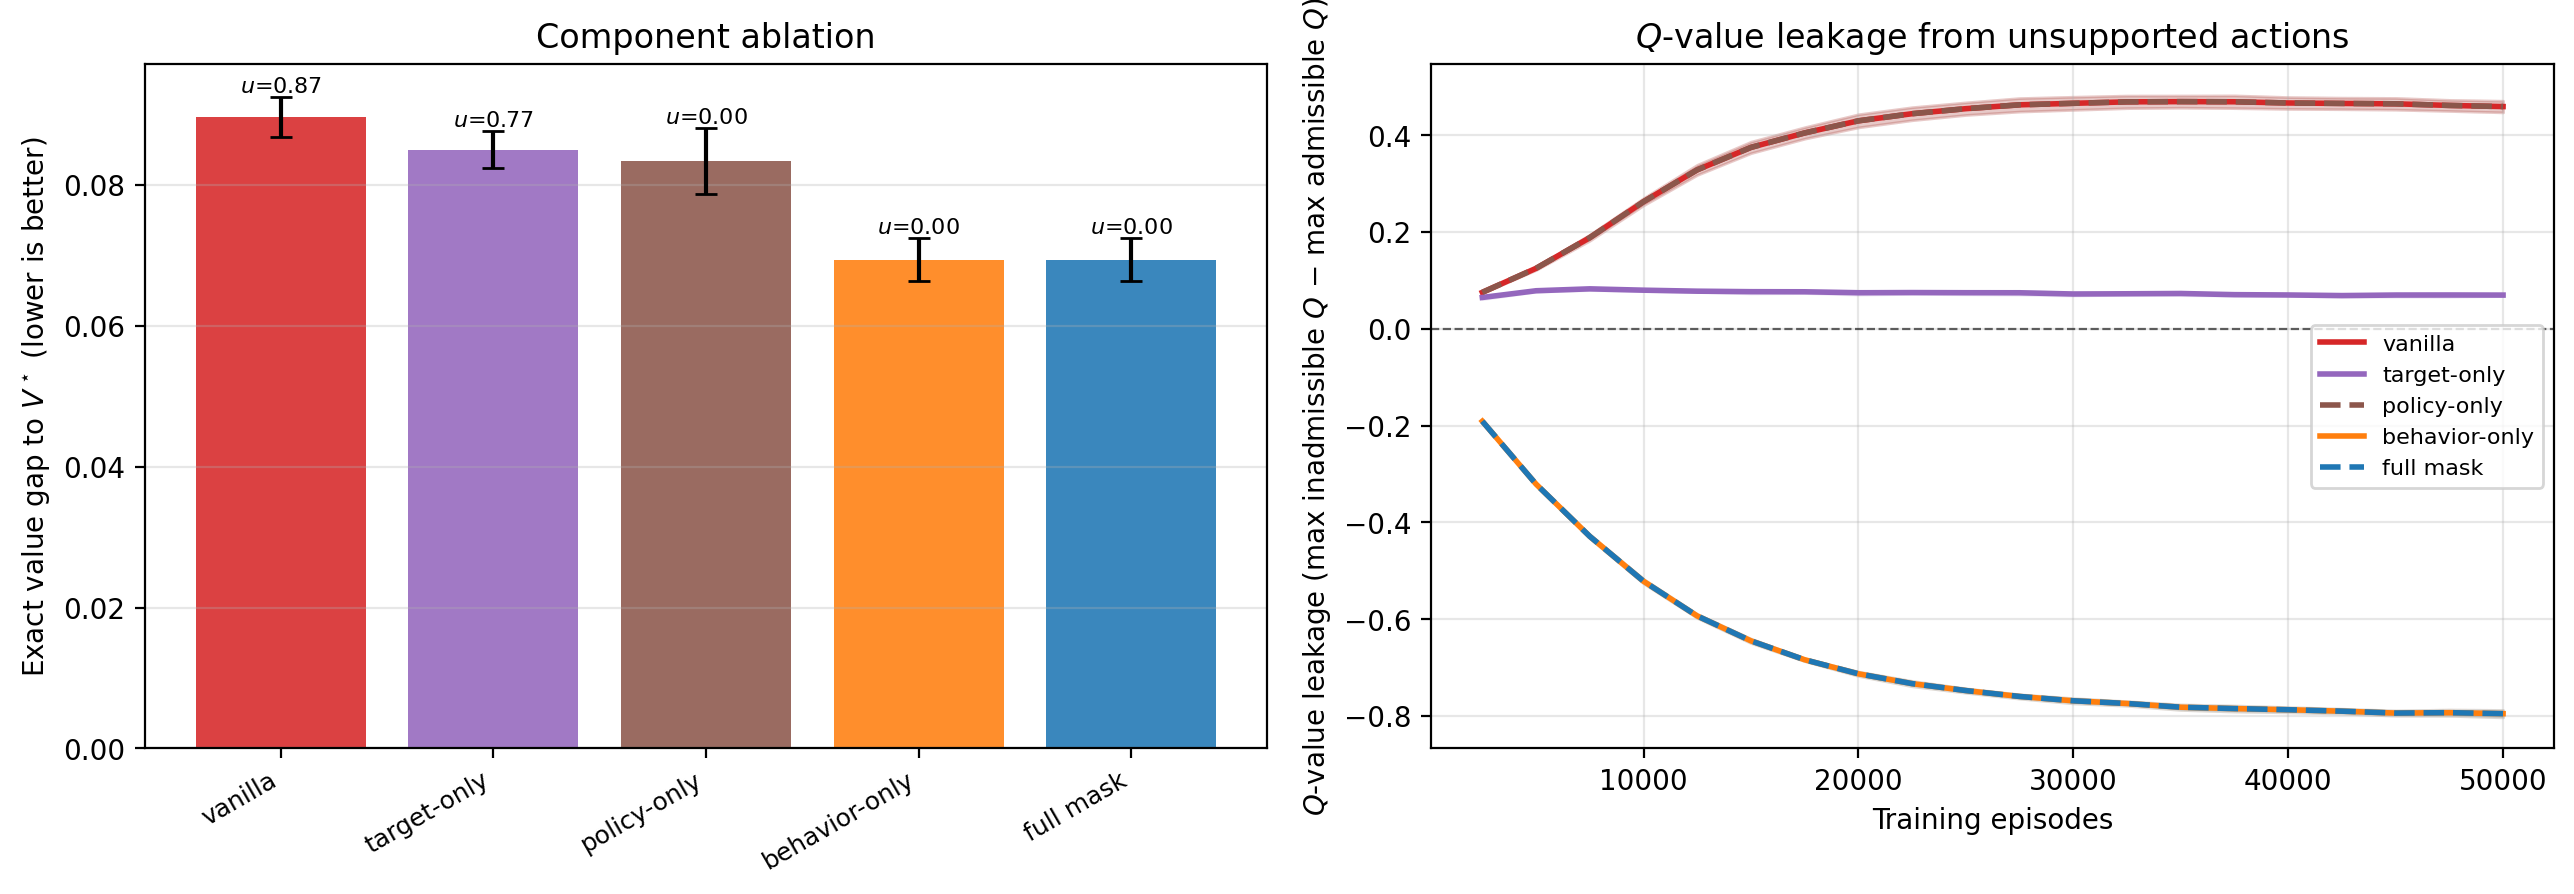
\includegraphics[width=0.95\linewidth]{component_ablation.png}
\caption{\textbf{Mechanism-level component ablation.}
Left: exact value gap to $V^\star$ for each masking location; numbers above bars
report the deployed unsupported-action rate $u$. Behavior-only masking matches
the full mask, while target-only and policy-only masking improve only marginally.
Right: $Q$-value leakage over training, defined as the gap between the best
inadmissible and best admissible action values. Policy-only masking leaves leakage
close to vanilla ($+0.46$), whereas behavior/full masking drives it negative
($-0.80$). Results use 5 seeds and $5{\times}10^4$ episodes; bars show $\pm$std and
bands show 95\% CI.}
\label{fig:ablation}
\end{figure}

\subsection{Remedy spectrum, online and cross-algorithm (Claim 3a)}
\label{sec:remedy}

\paragraph{From soft to hard (single-algorithm, $5{\times}10^4$ episodes).}
Support penalties reveal a support--value trade-off. Increasing $\lambda$ removes
deployed unsupported actions by $\lambda{=}1.0$, but the value gap plateaus around
$\dist\approx0.085$, above the hard-masking gap of $0.069$. CQL-style
conservatism is the strongest soft remedy we test ($\dist{=}0.080$ at
$\kappa{=}1$), but it still trails hard masking, and stronger conservatism
over-suppresses value ($\dist{=}0.089$ at $\kappa{=}2$;
App.~Fig.~\ref{fig:spectrum}).

\begin{figure}[tb]\centering
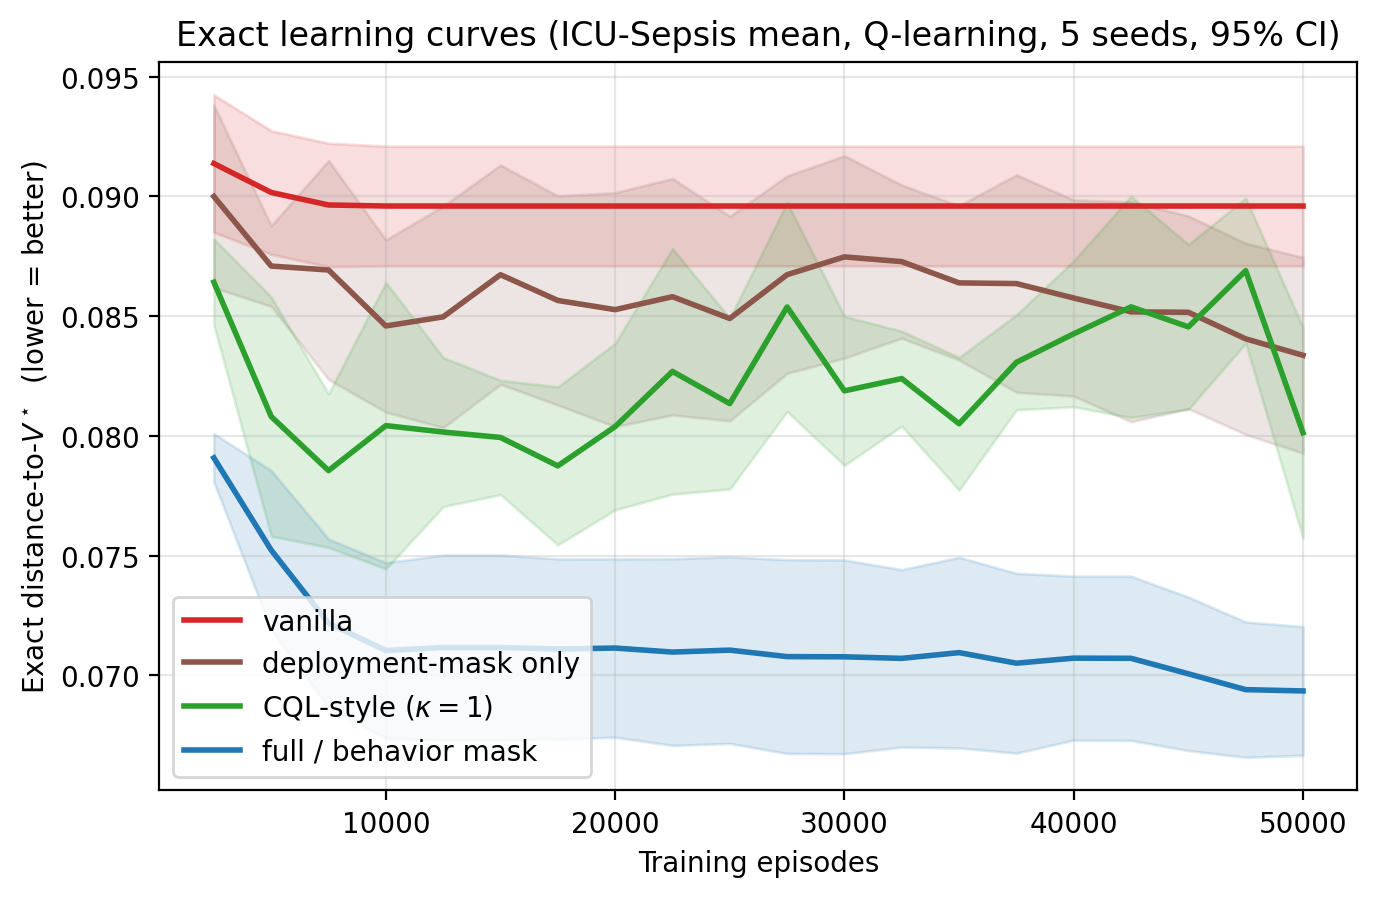
\includegraphics[width=0.60\linewidth]{exact_dist_curve.png}
\caption{Exact learning curves for policy snapshots over training
(5 seeds, 95\% CI). Values are computed as exact distance-to-$V^\star$, not
rollout return. The ordering matches the component ablation
(Table~\ref{tab:ablation}): vanilla and policy-only remain far from optimal,
CQL improves but trails hard masking, and behavior/full masking reach the best
plateau.}
\label{fig:exactcurve}
\end{figure}

\paragraph{Across algorithms and a model-based endpoint ($5{\times}10^5$ episodes).}
Table~\ref{tab:merged} reports the cross-algorithm picture, evaluated
\emph{exactly}. Admissibility masking improves all four model-free baselines,
with exact $\dist$ gains of $+0.014$ (Sarsa), $+0.014$ (Q-learning), $+0.026$
(DQN), and $+0.027$ (PPO).\footnote{We evaluate saved policies exactly against
the true dynamics; rollout-return learning curves are reported separately
(App.~Fig.~\ref{fig:rollouttiers}) for comparison with the benchmark metric.} At
the model-based endpoint, the admissibility-aware model-based agent (AA-MBRL)
reaches exact $J{=}0.874$ (gap $0.001$). We use this result as a diagnostic
endpoint rather than as a model-free comparison: once the benchmark's tabular
model structure and support labels are used, the remaining gap is almost entirely
closed. On a $716$-state tabular MDP, such model-based near-optimality is expected
\citep{auer2008ucrl,osband2013psrl}; the point is that the earlier gap is largely
an artifact of mean-imputation and unsupported-action handling.

\begin{table}[t]
\centering
\caption{Cross-algorithm breadth, \emph{exactly} evaluated. Policies are trained
for $5{\times}10^5$ episodes over 5 seeds and re-evaluated against the true
benchmark dynamics by exact value iteration to obtain $V^\pi$. Exact $J(\pi)$ is
reported as mean${\pm}$std for trained policies; $\dist$ is the exact
$d_0$-weighted value gap to $V^\star$; and ``Deploy unsupp.'' is the mean
unweighted fraction of non-terminal states in which the greedy deployed policy
selects $a\notin\Adm(s)$ (dashes mark reference policies for which it is not
reported).}
\label{tab:merged}
\begin{tabular}{llccc}
\toprule
Group & Method & Exact $J(\pi)\uparrow$ & $\dist\downarrow$ & Deploy unsupp. \\
\midrule
Reference & Random            & 0.780 & 0.095 & --- \\
          & Clinician         & 0.782 & 0.093 & --- \\
          & Optimal $J^\star$ & 0.875 & 0.000 & --- \\
\midrule
Base      & Sarsa       & $0.788{\pm}0.002$ & 0.087 & 0.83 \\
          & Q-learning  & $0.787{\pm}0.002$ & 0.088 & 0.85 \\
          & DQN         & $0.799{\pm}0.002$ & 0.076 & 0.79 \\
          & PPO         & $0.842{\pm}0.001$ & 0.033 & 0.58 \\
\midrule
+ support mask & AA-Sarsa   & $0.802{\pm}0.003$ & 0.073 & 0.00 \\
          & AA-Q        & $0.801{\pm}0.003$ & 0.074 & 0.00 \\
          & AA-DQN      & $0.826{\pm}0.003$ & 0.050 & 0.00 \\
          & AA-PPO      & $0.869{\pm}0.001$ & 0.006 & 0.00 \\
\midrule
+ support mask + model & AA-MBRL & $0.874{\pm}0.000$ & 0.001 & 0.00 \\
\bottomrule
\end{tabular}
\end{table}

\subsection{Remedy spectrum, offline finite-data (Claim 3b)}
\label{sec:offline}

We next ask whether the same support-handling issue appears in a finite-data
offline setting. We collect offline datasets of varying size $N$, where $N$
denotes the number of one-step transitions $(s_t,a_t,r_t,s_{t+1})$ sampled under
the clinician behavior policy. For each $N$, we build a certainty-equivalent
empirical model by treating the sampled transition frequencies as the MDP
dynamics, and compare three offline planners: \emph{naive} value iteration
with mean-imputation for actions unobserved in the $N$-sample dataset,
\emph{pessimistic} VI-LCB
\citep{jin2021pessimism,rashidinejad2021pessimism}, and
\emph{admissibility-masked} value iteration. All learned policies are evaluated
exactly against the true benchmark dynamics (Fig.~\ref{fig:offline}).

The support information available to each method differs. Pessimism infers
uncertainty from the $N$ samples through a count-based lower-confidence bonus over
observed actions, whereas masking uses the benchmark's oracle admissible set
$\Adm(s)$. Thus, the masked variant isolates the value of having known support
labels, while pessimism represents the more realistic case in which support must
be estimated from data.

Naive mean-imputation overestimates its own value by $+0.21$ at $N{=}10^5$, yet
its realized policy stagnates at $\dist\approx0.093$ across data sizes.
Pessimism remains calibrated (overestimation $\approx0$) and improves to
$\dist\approx0.069$. Oracle admissibility masking excludes unsupported actions
from planning and reaches $\dist\approx0.065$. Exact $V^\star$ is what makes this
overestimation pathology measurable---normally impossible in healthcare RL
\citep{gottesman2019guidelines}.

\begin{figure}[tb]\centering
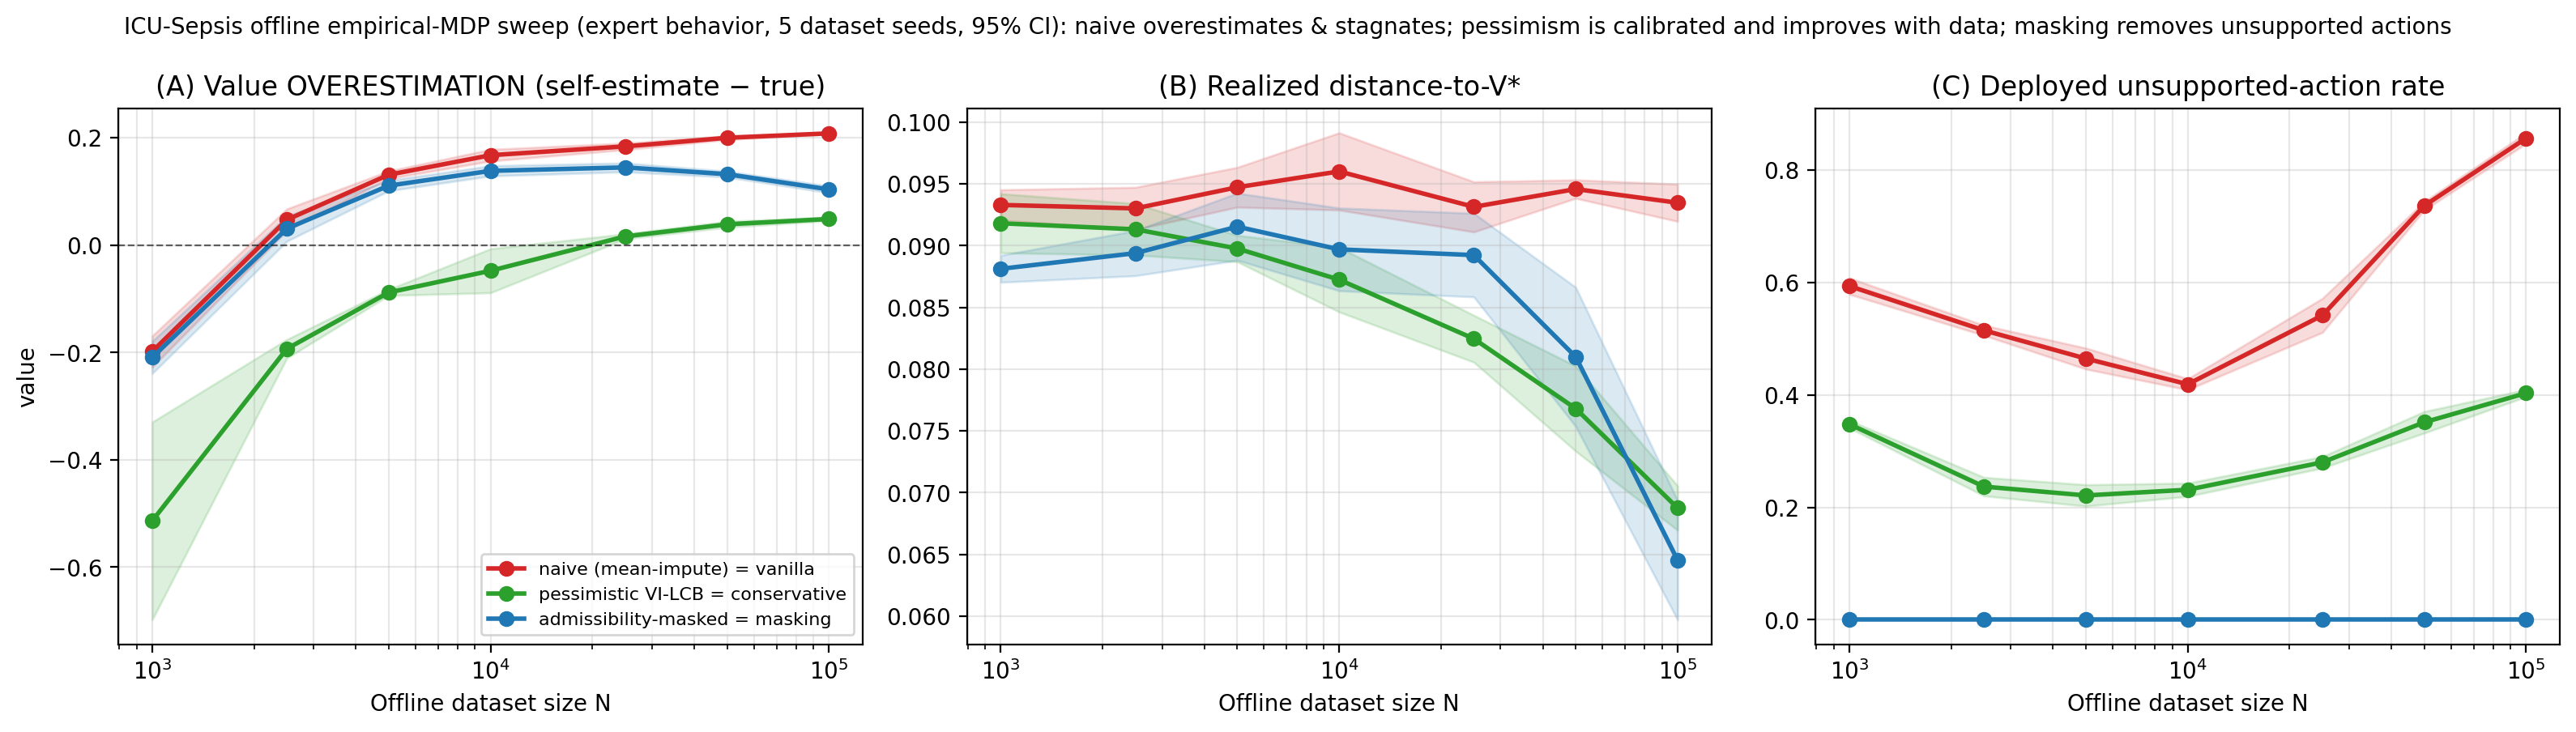
\includegraphics[width=0.95\linewidth]{offline_datasize.png}
\caption{Offline empirical-MDP sweep over dataset size $N$. Naive
mean-imputation overestimates its own value and its realized policy stagnates,
while pessimism and admissibility masking remain calibrated and improve with
data. Results use 5 seeds with 95\% CI; all policies are evaluated exactly
against the true $V^\star$.}
\label{fig:offline}
\end{figure}

\subsection{Supplementary robustness checks}
\label{sec:supp}

We move additional robustness checks to Appendix~\ref{app:figs} to keep the main
text focused on the mechanism. In brief, projecting the benchmark clinician policy, treated as a state-dependent
prior $\pi_E(a\mid s)$, onto $\Adm(s)$ removes most unsupported deployment while
preserving value; the failure
is specific to the \texttt{mean} strategy rather than the \texttt{terminate}
strategy; and ICU-Sepsis has no dead-end states
\citep{fatemi2021deadends} under the exact model. These checks are supportive
rather than load-bearing for the central claim that behavior-level support
control is the key intervention.

% =============================================================================
\section{Discussion}
\label{sec:discussion}
\paragraph{Why survival rate hides the failure.}
Survival values in ICU-Sepsis occupy a narrow range: Random and clinician policies
are already around $0.78$, while the optimal value is $0.875$. When unsupported
actions are mean-imputed to behave like random admissible actions, a policy can
achieve a plausible survival rate while still choosing unsupported actions in most
states. This is why survival rate alone is not diagnostic. The mechanism is only
visible when value is paired with support-aware diagnostics such as $\dist$,
deployed unsupported-action rate, and $Q$-value leakage.

\paragraph{What transfers beyond the benchmark.}
Our numerical gap-closing results are benchmark-internal. They rely on the fact
that ICU-Sepsis treats its estimated tabular dynamics as ground truth and exposes
an exact $V^\star$; real clinical cohorts do not provide such a ruler. The
transferable lesson is therefore not that admissibility masking is a deployable
clinical policy, but that data-unsupported actions should be handled explicitly
and pessimistically rather than silently mean-imputed. The finite-data offline
study reinforces this point: naive mean imputation overestimates its own value,
whereas pessimism and masking remain calibrated.

\paragraph{Benchmark guidance.}
Future ICU-Sepsis reports should make action-support handling explicit. At minimum,
we recommend reporting the imputation or masking strategy, the deployed
unsupported-action rate, the exact value gap to $V^\star$, and either $Q$-value
leakage or offline value overestimation. These metrics turn a hidden benchmark
default into an auditable modeling choice.

\paragraph{Significance for offline medical RL.}
Offline medical RL learns from logged data with uneven action coverage. Our study
uses ICU-Sepsis as a controlled measurement instrument to show how a seemingly
benign imputation rule can change learned behavior. The result is a methodological
caution and an evaluation protocol, not a clinical recommendation.

% =============================================================================
\section{Limitations}
\label{sec:limitations}
Our study is benchmark-internal and tabular: ``unsupported'' means insufficient data
support, not medical incorrectness, and we make no clinical claims. Whether the
mean-imputation failure and the behavior-masking fix transfer to high-dimensional,
continuous-action, or clinically realistic function-approximation settings is
untested; in particular we do not evaluate continuous-control algorithms such as
SAC, and the DQN/PPO agents we include remain confined to the small discrete
ICU-Sepsis benchmark. The offline empirical-MDP sweep is a step toward the
realistic finite-data regime but remains tabular. We use 5 seeds (effect
sizes for the support diagnostics are large, e.g.\ 87\%$\to$0\% deployed unsupported
and leakage $+0.46\to-0.80$). The clinician policy itself is not fully
admissibility-respecting, a property of the benchmark we inherit.

% =============================================================================
\section{Conclusion}
\label{sec:conclusion}
ICU-Sepsis's default mean-imputation makes data-unsupported actions look average, so
model-free agents adopt them at a value cost that survival rate hides. Using the
benchmark's exact $V^\star$, we localize the failure to behavior-level sampling,
explain it through an exact $Q$-value-leakage diagnostic, and compare support-aware
remedies online, across algorithms, and offline. Inadmissible-action handling should
be reported, not left to a hidden default: the gap is largely an artifact of
mean-imputation, and the benchmark already exposes the support information needed to
diagnose and mitigate it.

% =============================================================================
\paragraph{Reproducibility statement.}
All mechanism diagnostics reproduce from the released one-command scripts---exact value
iteration on the shipped ICU-Sepsis dynamics (metric definitions in \S\ref{sec:method});
the cross-algorithm and model-based results (Table~\ref{tab:merged}) are exact
evaluations of the saved policies against the true dynamics with the same script.
Code and saved policies are available at
\url{https://anonymous.4open.science/r/icu-sepsis-ood-supplement-0DC8/}.

\bibliographystyle{plainnat}
\bibliography{references}

\clearpage
% =============================================================================
\appendix
\raggedbottom  % appendix-local: don't stretch glue on under-full [H]-float pages
\section{Supplementary figures}
\label{app:figs}
This appendix collects supplementary figures omitted from the main text.
Fig.~\ref{fig:rollouttiers} reports benchmark-style rollout-return learning
curves for comparability with the original benchmark metric, whereas
Figs.~\ref{fig:spectrum}--\ref{fig:deadend} use the paper's exact-evaluation
diagnostics unless stated otherwise. These figures include the penalty-sweep
remedy analysis and the supplementary checks discussed in \S\ref{sec:supp}
(expert projection, robustness across algorithms and imputation strategies, and
dead-end structure).

\begin{figure}[H]\centering
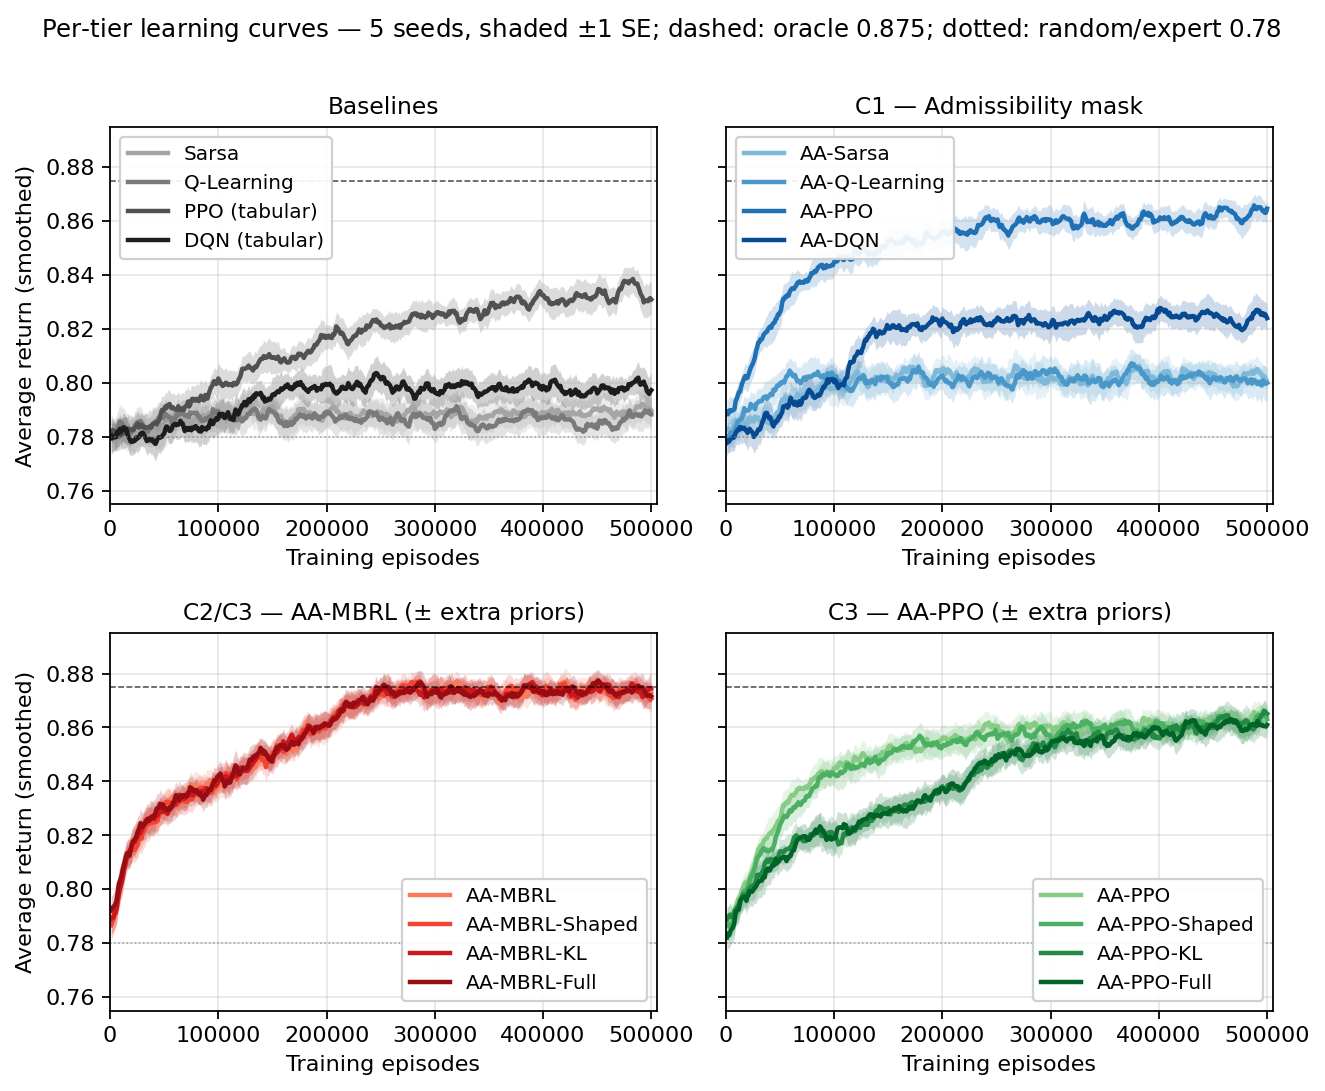
\includegraphics[width=0.95\linewidth]{fig1_return_tiers.png}
\caption{\textbf{Benchmark rollout-return learning curves.}
Per-tier average return---the benchmark's standard last-$1000$-episode
mean---vs.\ training episodes ($5{\times}10^5$ episodes, 5 seeds, $\pm$1 SE;
dashed: oracle $0.875$, dotted: random/clinician $0.78$). This rollout axis is
shown only for comparability with prior benchmark reporting and differs from the
exact $V^\pi$-based evaluation used in the main text (cf.\ Fig.~\ref{fig:exactcurve}
and Table~\ref{tab:merged}). Because rollout estimates are noisy, some
near-optimal cells can exceed $V^\star$ on this axis; the corresponding final
policies are exact-evaluated in Table~\ref{tab:merged}.}
\label{fig:rollouttiers}
\end{figure}

\begin{figure}[H]\centering
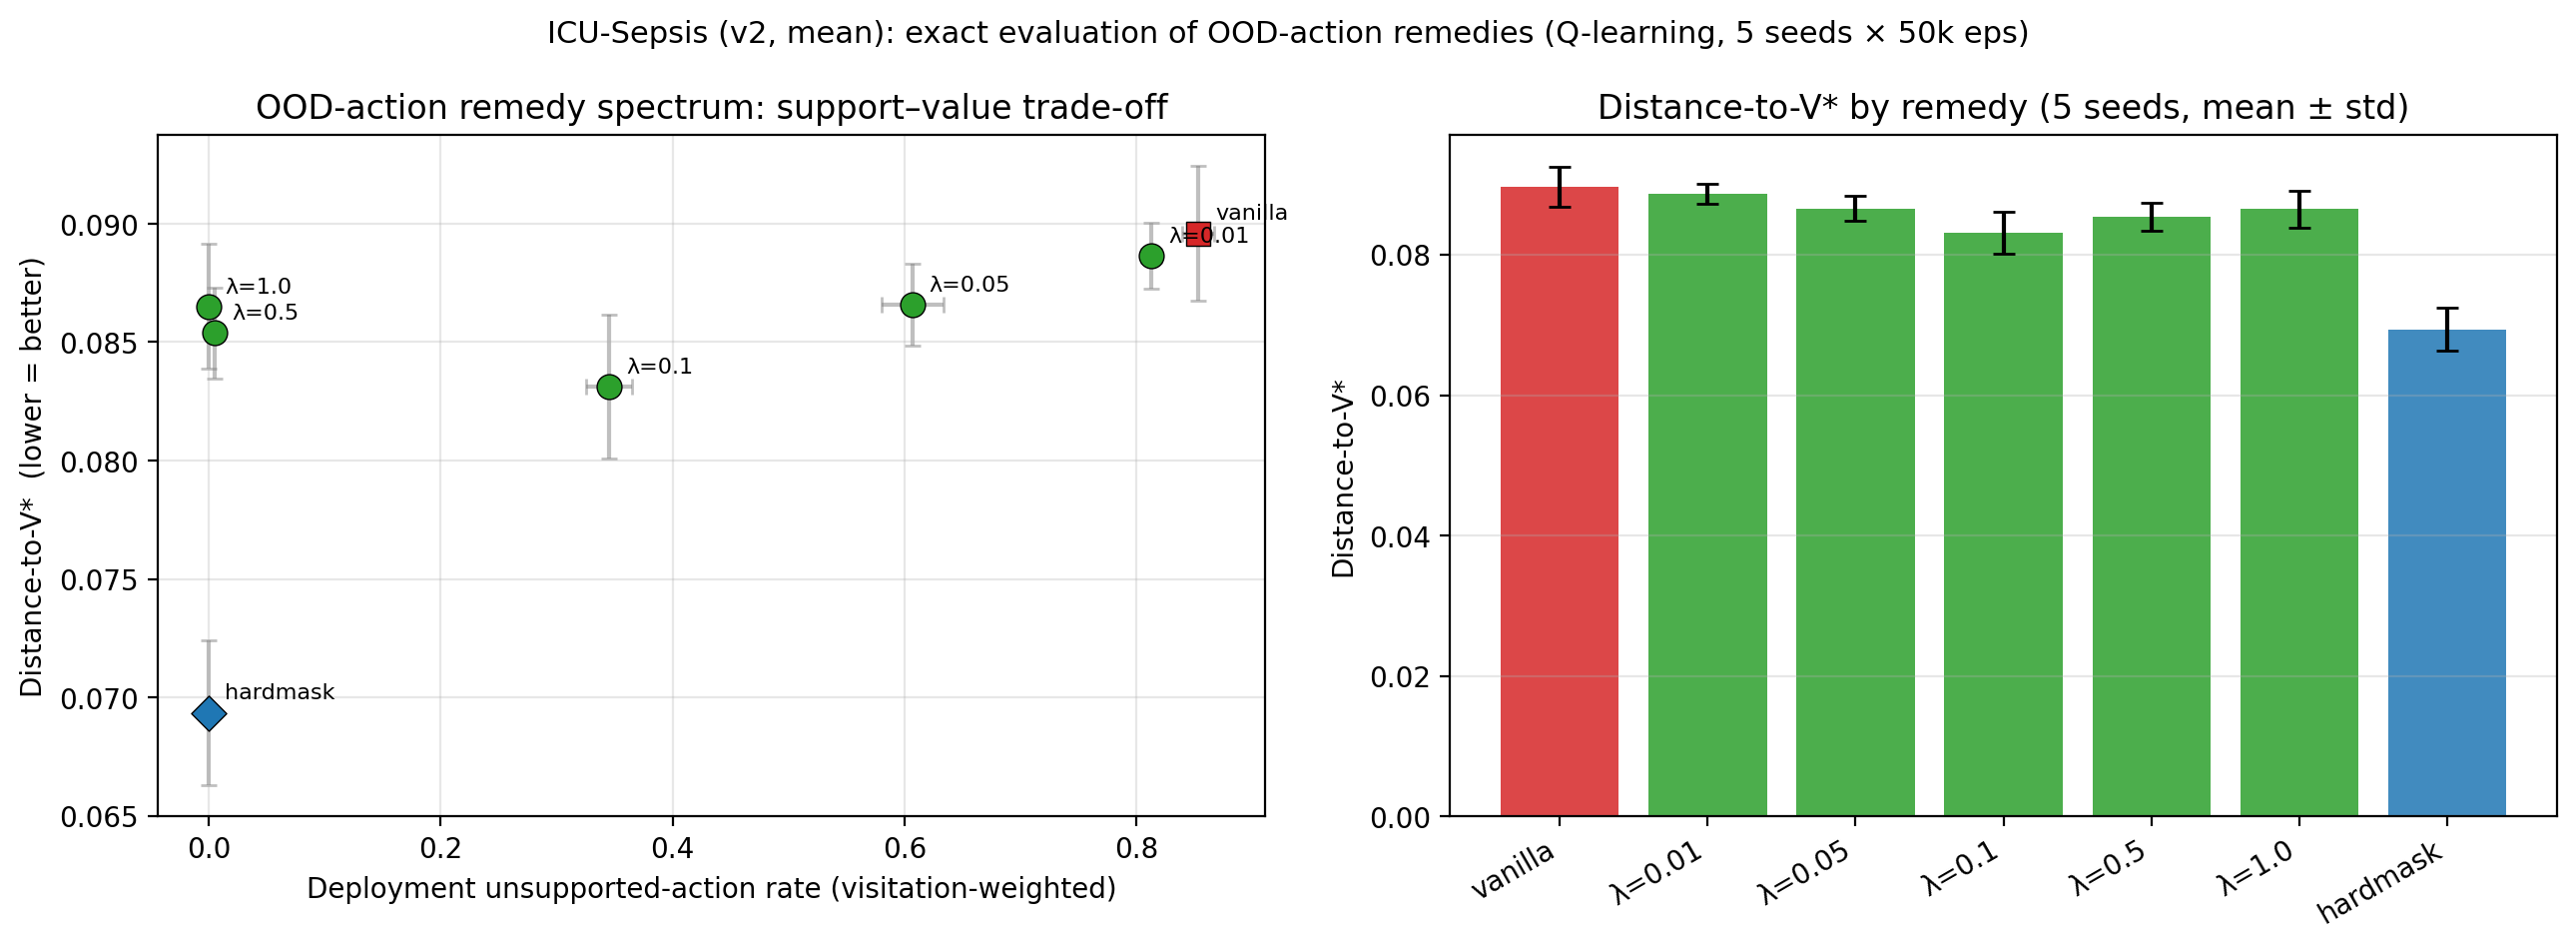
\includegraphics[width=0.85\linewidth]{penalty_tradeoff.png}
\caption{Remedy spectrum (penalty sweep): increasing the penalty removes
unsupported actions but plateaus in $\dist$, whereas hard masking achieves the
lowest value gap among these remedies (5 seeds, $5{\times}10^4$ episodes;
error bars show $\pm$std).}
\label{fig:spectrum}
\end{figure}

\paragraph{Expert projection (Fig.~\ref{fig:expert}).}
For the expert-projection check we treat the benchmark clinician policy as a
state-dependent prior $\pi_E(a\mid s)$ and guide exploration with its
admissibility-projected form
\[
\pi_E^{\Adm}(a\mid s)=\frac{\pi_E(a\mid s)\,\mathbf{1}\{a\in\Adm(s)\}}
{\sum_{a'\in\Adm(s)}\pi_E(a'\mid s)},
\]
so exploration never injects unsupported actions. This is a supplementary
diagnostic, not a proposed clinical policy.

\begin{figure}[H]\centering
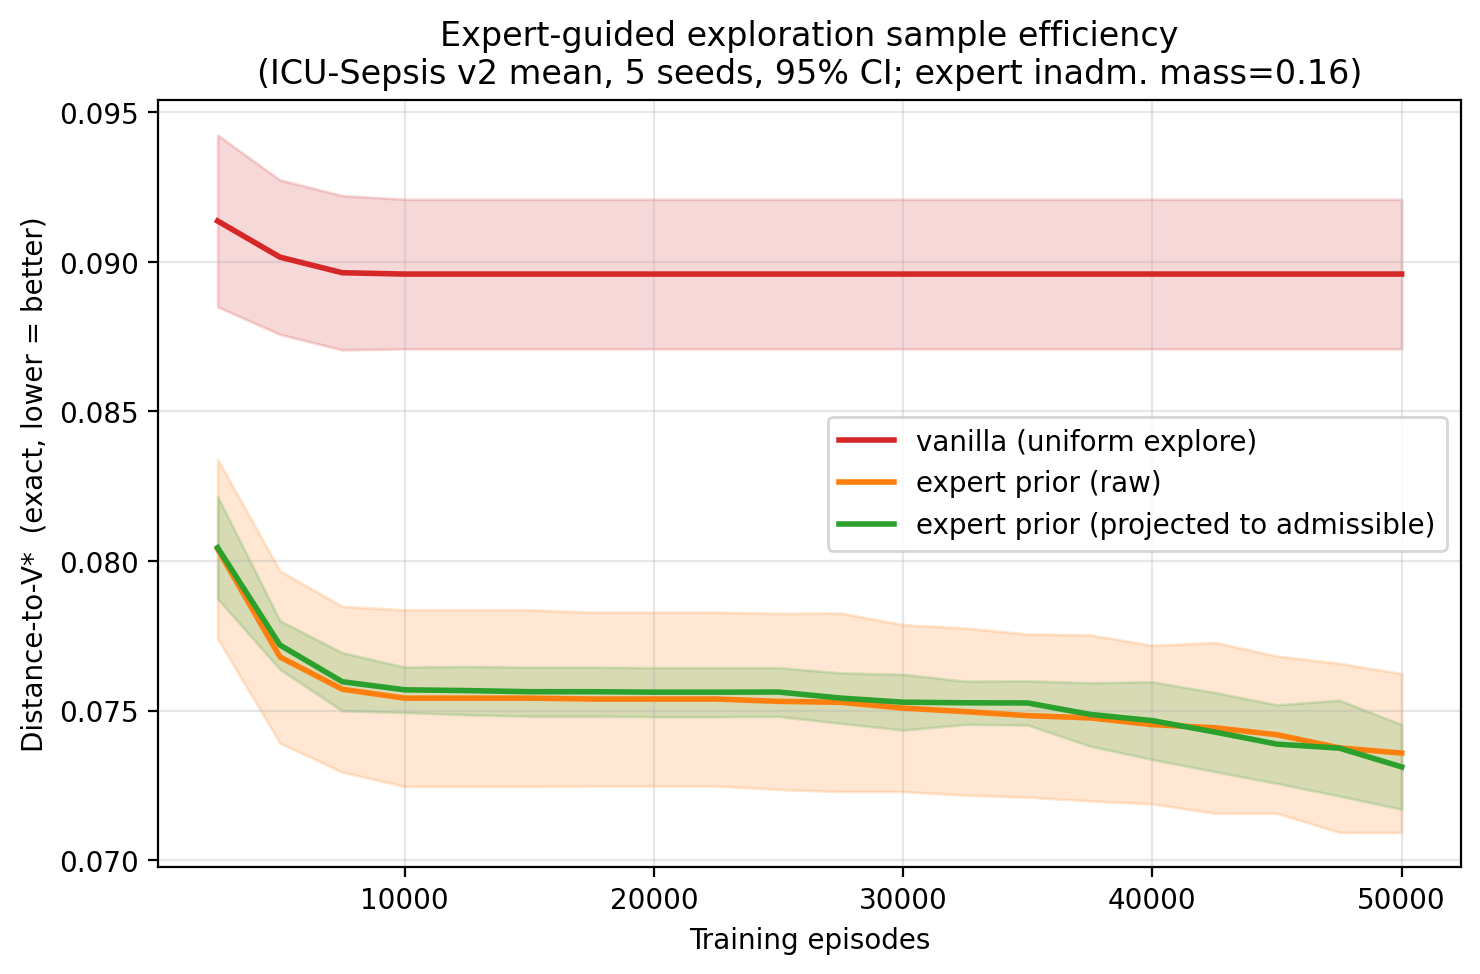
\includegraphics[width=0.6\linewidth]{expert_prior_curve.png}
\caption{Expert-guided exploration. Projecting the clinician prior onto
$\Adm(s)$ nearly eliminates unsupported deployment ($0.5\%$) while preserving
value, showing that support projection can reduce unsupported deployment without
destroying the expert-guided signal (5 seeds, $5{\times}10^4$ episodes;
bands show 95\% CI).}
\label{fig:expert}
\end{figure}

\begin{figure}[H]\centering
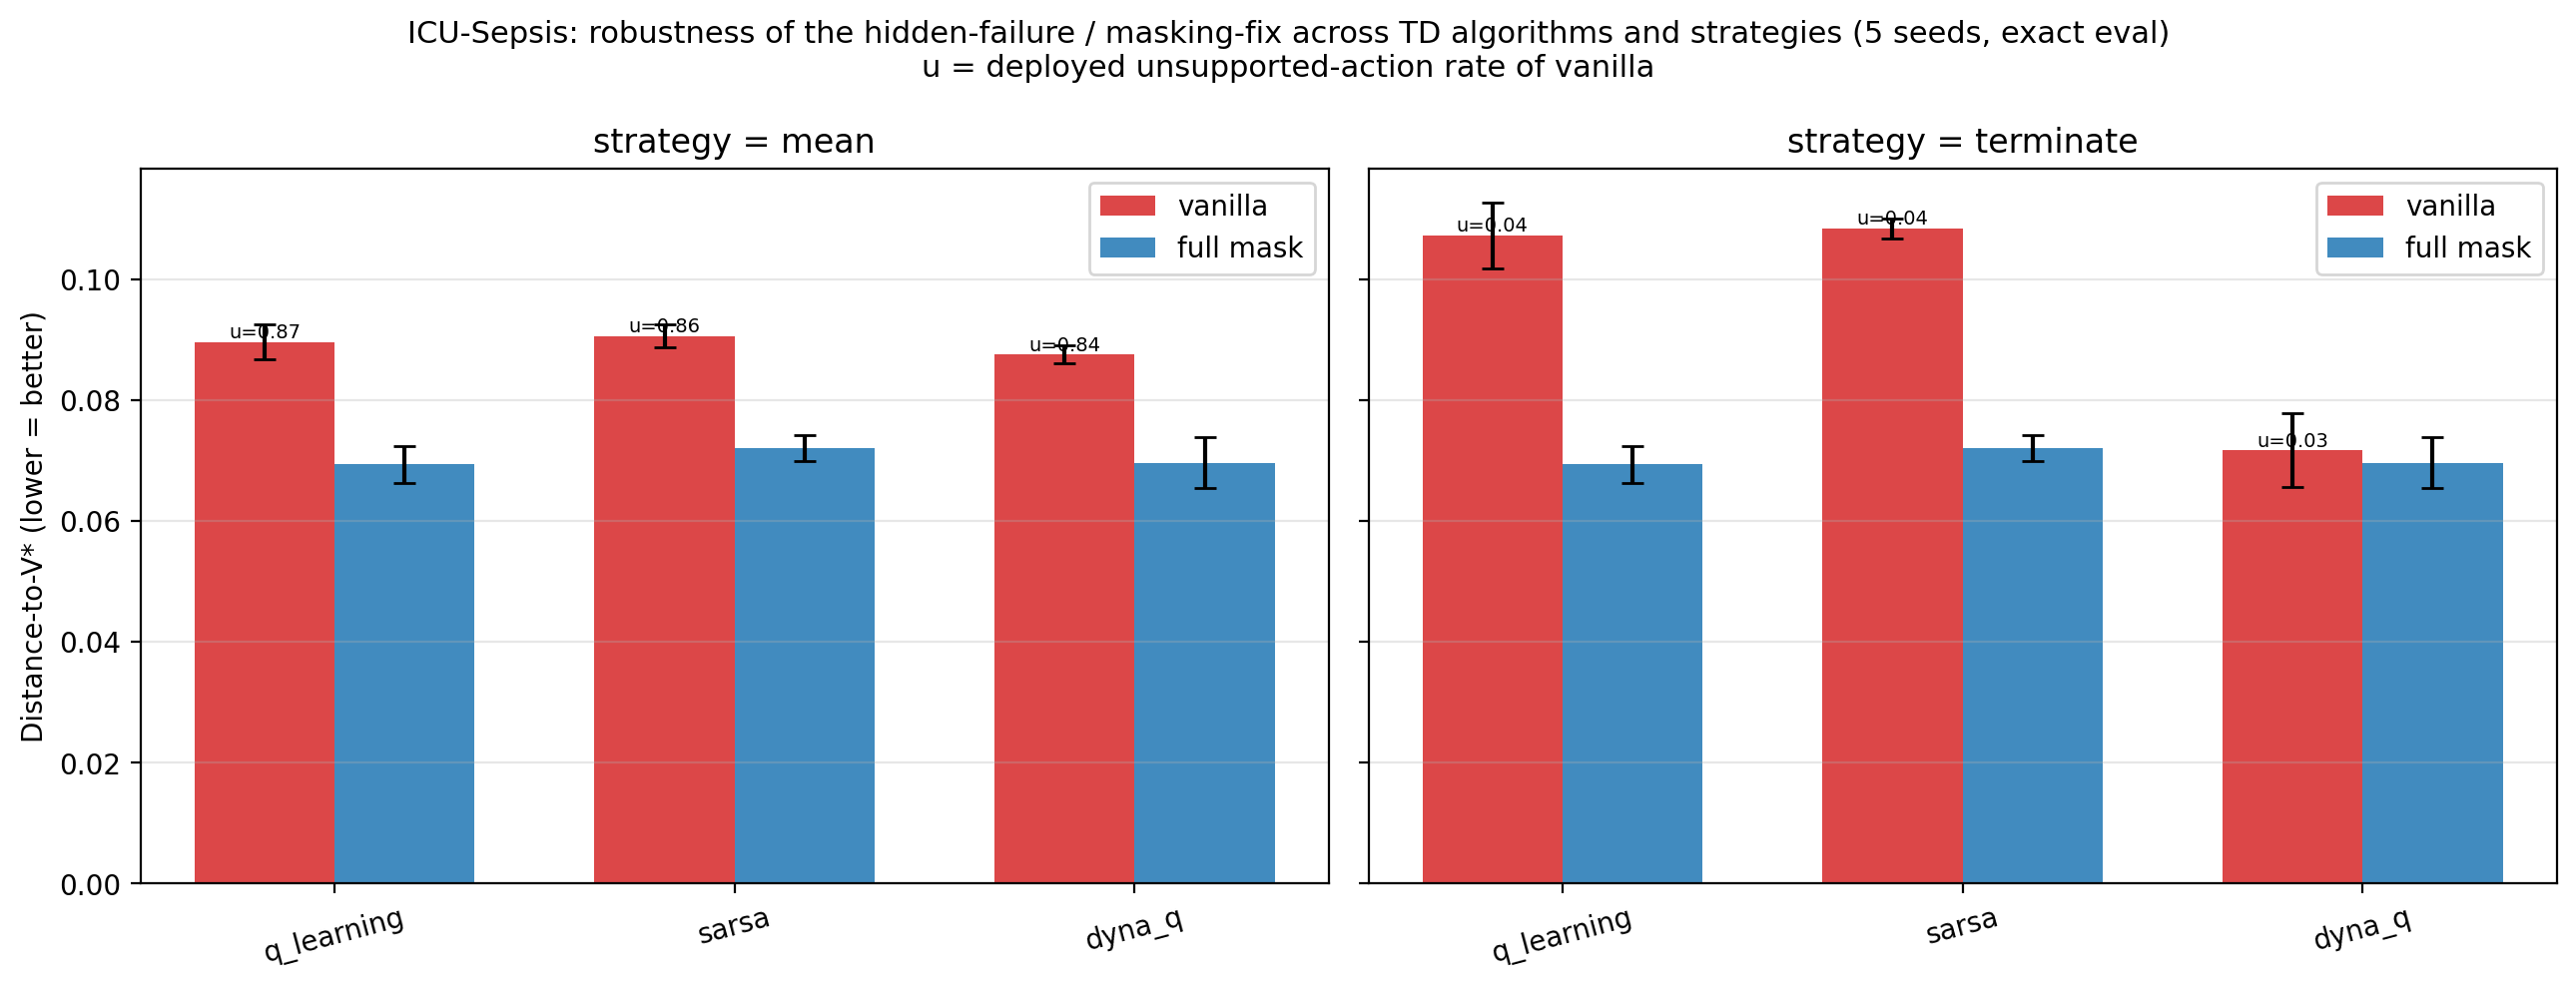
\includegraphics[width=0.95\linewidth]{robustness.png}
\caption{Robustness across tabular TD algorithms and imputation strategies,
exactly evaluated by distance-to-$V^\star$. Across Q-learning, Sarsa, and
Dyna-Q, full masking improves or matches vanilla under both the \texttt{mean}
and \texttt{terminate} strategies. Numbers above red bars report the deployed
unsupported-action rate of vanilla. Results use 5 seeds and
$5{\times}10^4$ episodes; error bars show $\pm$std.}
\label{fig:robust}
\end{figure}

\begin{figure}[H]\centering
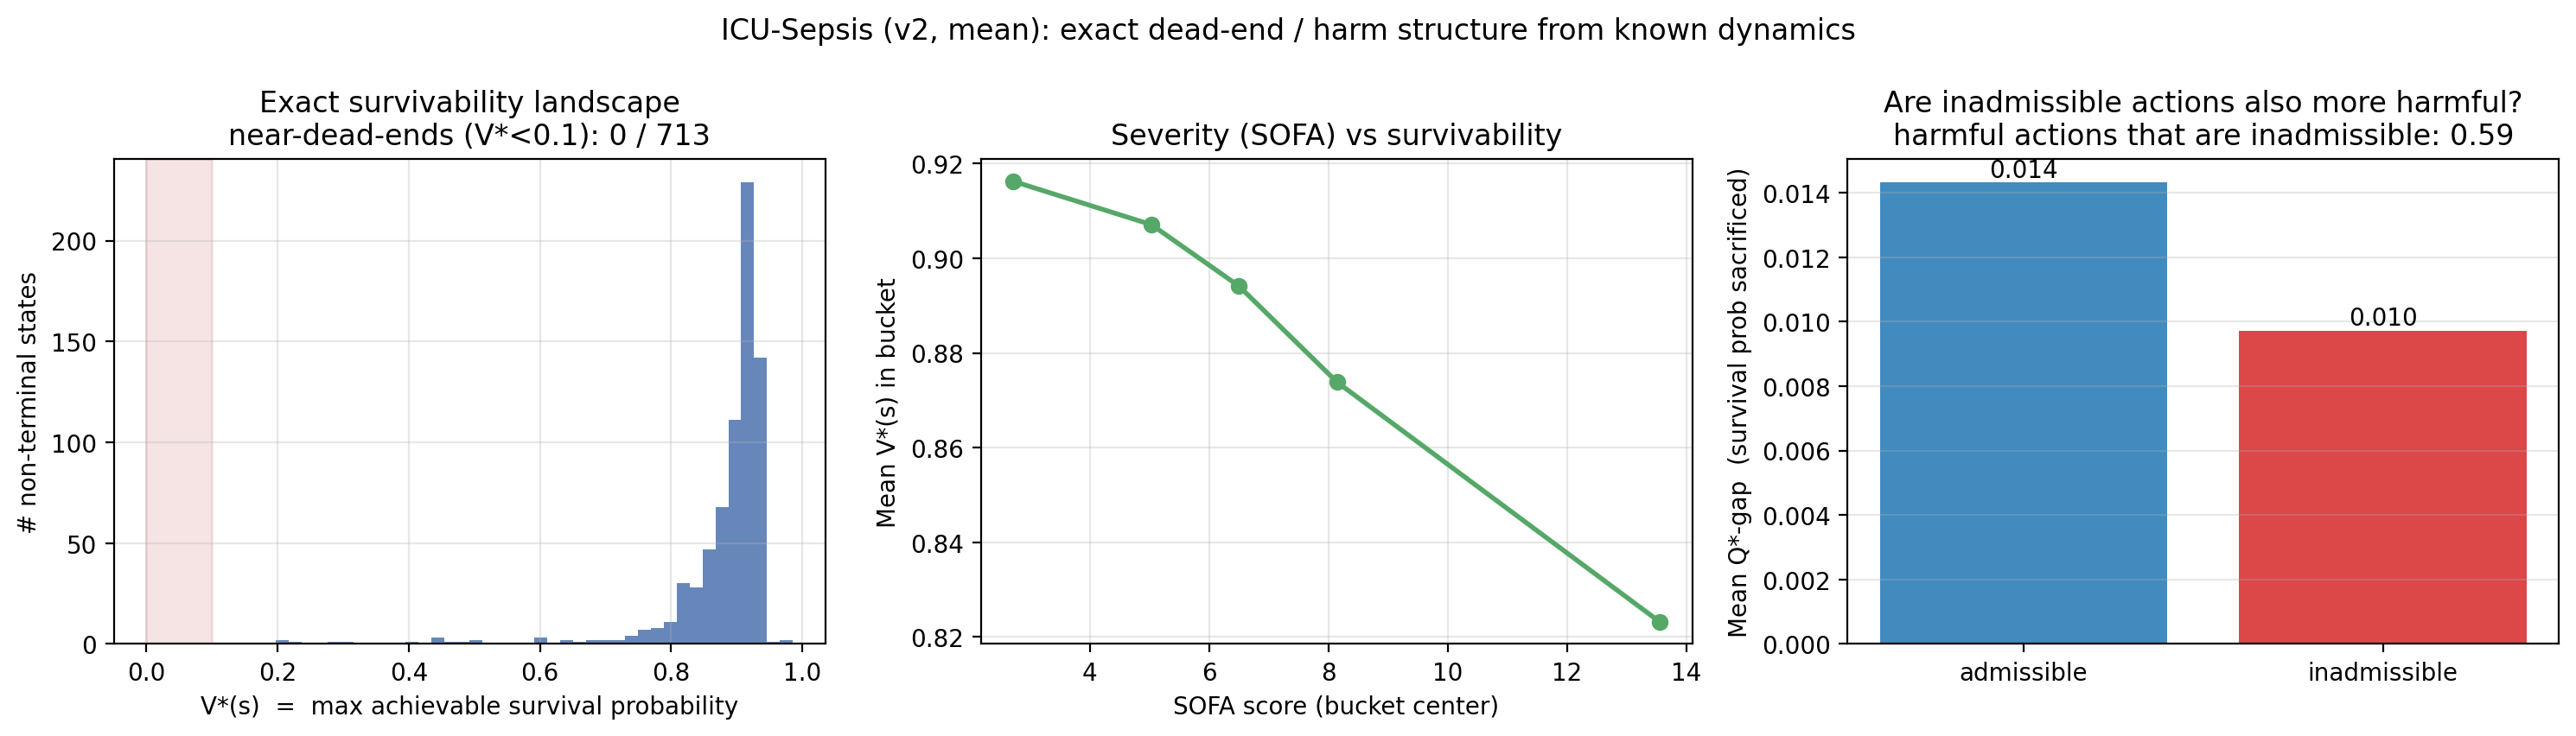
\includegraphics[width=0.95\linewidth]{deadend_structure.png}
\caption{Dead-end analysis under the exact ICU-Sepsis model. No non-terminal
state has zero optimal survival probability ($\min_s V^\star(s)=0.198$), so the
benchmark contains no dead-end states under the criterion of
\citet{fatemi2021deadends}; 427/713 patient states have $V^\star(s)>0.9$.}
\label{fig:deadend}
\end{figure}

% NeurIPS paper checklist. Lives in checklist.tex (this folder); answers filled in.
\newpage
\input{checklist.tex}
\end{document}